%!TeX root=../tese.tex
%("dica" para o editor de texto: este arquivo é parte de um documento maior)

% Conteúdo da subseção sobre Inserção de Usuários
% Este arquivo é importado em 02-implementacao.tex

O processo de recrutamento de participantes para o piloto BikeSP iniciou-se com ampla divulgação midiática (entrevistas em jornais, redes sociais, site institucional), direcionando interessados para formulário online hospedado em instância LimeSurvey na NuvemUSP. O formulário coletava: dados pessoais (nome, CPF, email, data de nascimento, gênero), número do Bilhete Único (pré-requisito para participação, pois remuneração seria creditada neste cartão), senha para acesso ao aplicativo móvel, endereços textuais de até três localizações (tipicamente casa e trabalho/escola), telefone para contato, e concordância com Termo de Consentimento Livre e Esclarecido (TCLE --- documento obrigatório aprovado por Comitê de Ética para pesquisas envolvendo seres humanos). Durante o período de inscrições, o formulário recebeu aproximadamente 3.000 submissões, volume que requeria automação para transferência ao banco de dados PostgreSQL do sistema BikeSP.

A funcionalidade de inserção em lote, acessível via botão ``Inserir Usuários!'' no painel administrativo, executa script que: (i) conecta à API do LimeSurvey e baixa todas respostas ainda não processadas; (ii) itera sobre cada resposta aplicando validações (CPF válido via algoritmo de verificação de dígitos, email em formato correto e único no sistema, Bilhete Único com 15 dígitos numéricos, senha com mínimo de caracteres configurável); (iii) criptografa a senha antes de armazenar (segurança crítica); (iv) geocodifica endereços textuais chamando APIs externas (TomTom, Google Maps, Nominatim OSM) para converter em coordenadas GPS; (v) armazena dados cadastrais da pessoa, vinculação do cartão Bilhete Único com status ativo, e coordenadas de casa e trabalho; (vi) atribui participante a coorte inicial (pode ser randomizado ou seguir configuração padrão); e (vii) registra logs detalhados de sucesso/falha para cada usuário processado.

Execução ocorre em thread separada (processamento assíncrono) para não bloquear interface administrativa durante operação (geocodificação via APIs externas é o gargalo principal). Botão fica desabilitado durante processamento, prevenindo cliques duplos que iniciariam múltiplas execuções simultâneas. Mensagem inicial ``Usuários novos estão sendo inseridos!'' confirma início; mensagem final reporta quantidade inserida (``X usuários inseridos com sucesso'') ou erros encontrados. A Figura~\ref{fig:insercao_usuarios} mostra a interface desta funcionalidade.

\begin{figure}[H]
  \centering
  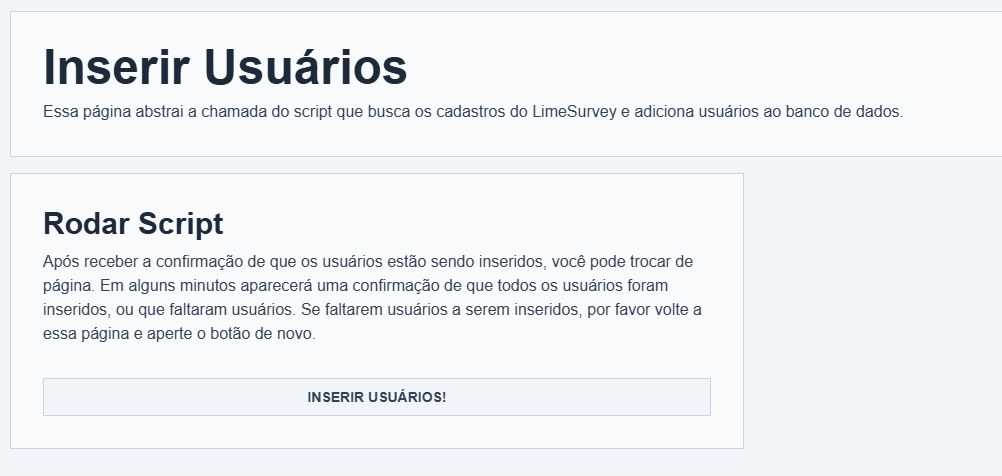
\includegraphics[width=0.95\textwidth]{figuras/inserir_usuarios.PNG}
  \caption{Interface de inserção de usuários no painel administrativo, com botão para executar o script de importação do LimeSurvey.}
  \label{fig:insercao_usuarios}
\end{figure}

O sistema implementa verificação de CPF existente antes de tentar inserção, prevenindo duplicações mesmo se script executado múltiplas vezes sobre mesmas respostas do LimeSurvey (comportamento idempotente). Quando endereço falha em geocodificação (10-20\% dos casos conforme discussão na subseção de Localizações), localização é criada marcada como ``inválida'', permitindo participante existir no sistema mas impedindo uso daquela localização em viagens até correção manual via interface administrativa. Esta estratégia parcialmente otimista (criar usuário mesmo com dados incompletos) prioriza não bloquear participação --- melhor ter usuário com localização a corrigir que rejeitar inscrição completamente. Mensagens de aviso (``Y usuários faltaram a serem inseridos'', ``Z endereços não puderam ser geocodificados'') orientam reexecução do script (para tentar novamente usuários que falharam transientemente) e correção manual de localizações.

Embora o formulário LimeSurvey coletasse aproximadamente 3.000 inscrições, apenas 1.217 participantes foram efetivamente inseridos no sistema e incluídos no piloto. Critérios de elegibilidade aplicados durante seleção (manualmente por economistas antes de liberar CPFs para script de inserção) incluíam: residência em São Paulo (verificação via CEP), posse de Bilhete Único ativo, não ser cicloativista regular (auto-declaração --- para evitar viés de seleção, experimento buscava medir impacto em usuários representativos, não entusiastas pré-dispostos), e disponibilidade para participar durante seis meses. Preferência adicional para diversidade de perfis socioeconômicos e geográficos. Esta separação entre coleta ampla pelo LimeSurvey e inserção seletiva pelo script permitiu flexibilidade experimental mantendo integridade metodológica.

A primeira execução do script, inserindo ~1.200 usuários simultaneamente, foi coordenada com atribuição inicial de coortes via funcionalidade de upload em lote (descrita na subseção de Coortes). Workflow combinado: economistas geravam CSV com (CPF, ID\_Coorte) aplicando randomização estratificada; administrador executava script de inserção LimeSurvey→PostgreSQL; aguardava confirmação de sucesso; executava upload de atribuição de coortes; verificava balanceamento (~400 usuários por coorte); enviava notificações de boas-vindas via sistema de notificações. Este processo único e crítico ocorreu na véspera do início oficial do piloto, requirendo coordenação temporal precisa para permitir resolução de problemas antes que participantes recebessem instruções para ativar o aplicativo.

Este processo de inserção em lote via script administrativo foi desenvolvido exclusivamente para o projeto piloto, onde era necessário selecionar manualmente 1.217 participantes dentre 3.000 inscritos aplicando critérios de elegibilidade (residência em São Paulo, não ser cicloativista, diversidade socioeconômica). O formulário LimeSurvey serviu como porta de entrada ampla para candidatos, enquanto o script de inserção permitia controle fino sobre quem seria efetivamente incluído no experimento controlado.

Para a implementação municipal em larga escala (10.000-50.000 usuários), quando o programa BikeSP for liberado para todos os ciclistas de São Paulo, esta arquitetura de duas etapas (LimeSurvey → script → banco de dados) seria substituída por cadastro direto e automático via aplicativo móvel. Usuários interessados instalariam o aplicativo, preencheriam dados cadastrais diretamente na interface, e seriam automaticamente integrados ao sistema sem necessidade de aprovação ou processamento em lote por administradores. O formulário LimeSurvey e o script de inserção foram ferramentas necessárias apenas para o contexto experimental do piloto, não fazendo parte da arquitetura planejada para a política pública permanente.


